\subsection{Opgave 1 - Half-adder}
\begin{enumerate}
	\item[1)]
	Architecture body i VHDL kan skrives på tre forskellige måder; dataflow, behavioral og structural. \\
	Half-adder beskrives i Dataflow style ved hjælp af direkte implementering af logiske gates. Skrivemåden gør det nemt at overføre programmet direkte til hardware og de logiske gates. \\
	I Behavioral style opskrives half-adderen ved brug af if/else statements. Dette giver en god forståelse af selve half-adderens funktion, men det er kompliceret at overføre det til logiske gates ud fra kodens syntax. \\
	I structural style laves et miks af de to ovenstående, da der først defineres en funktion for hver logisk gate som det ses i dataflow style, og derefter implementeres funktionerne i halfadder entity’en. Denne style er god at bruge, hvis man skal implementere en funktion flere gange.\\
	\item[2)]
	Et RTL view af de tre forskellige måder at skrive en half-adder på, giver følgende forskellige resultater:\\
\begin{figure}[h]
	\centering
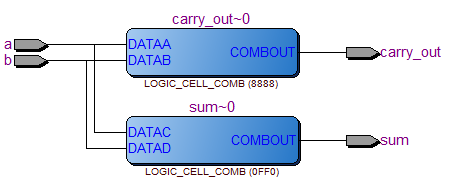
\includegraphics[scale=0.8]{pictures/Oevelse1/Half_adder/Behavioral.JPG}
\caption{Half-adder - Behavioral RTL view}
\label{fig:HaBehavioralRTL}
\end{figure}

\begin{figure}[h]
	\centering
	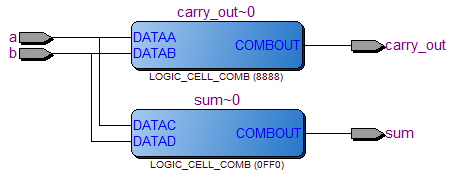
\includegraphics[scale=0.8]{pictures/Oevelse1/Half_adder/dataflow.JPG}
	\caption{Half-adder - Dataflow RTL view}
	\label{fig:HaDataflowRTL}
\end{figure}

\begin{figure}[h]
	\centering
	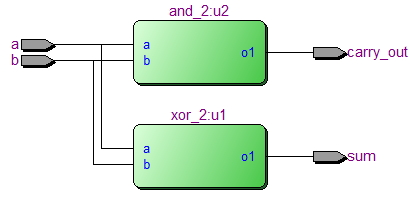
\includegraphics[scale=0.8]{pictures/Oevelse1/Half_adder/Structural.JPG}
	\caption{Half-adder - Structural RTL view}
	\label{fig:HaStructuralRTL}
\end{figure}
	\newpage
	
	Ud fra ovenstående figurer ses det, at dataflow-style og behavioral-style "afkodes" på samme vis, hvor de blå bokse symboliserer en logisk funktion. I structural-style angiver de grønne bokse, også logiske funktioner, men disse er defineret af os, som hhv en AND-funktion og en XOR-funktion. Det er altså med structural-style at vi nemmest kan se, hvilke gates vi skal bruge i en fysisk opbygning af systemet.\\

	\item[3)]
	Følgende tre figurer viser en Timing simulation af hver style. \\
\begin{figure}[h]
	\centering
	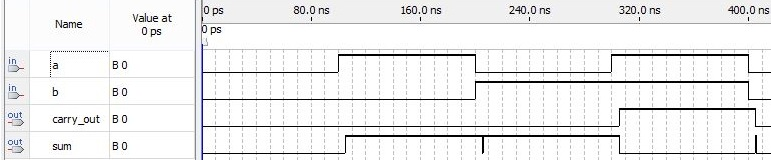
\includegraphics[scale=0.6]{pictures/Oevelse1/Half_adder/Behavioral_timing_simulation.jpg}
	\caption{Half-adder - Behavioral Timing Simulation}
	\label{fig:HaBehavioralTimingSim}
\end{figure}
\begin{figure}[h]
	\centering
	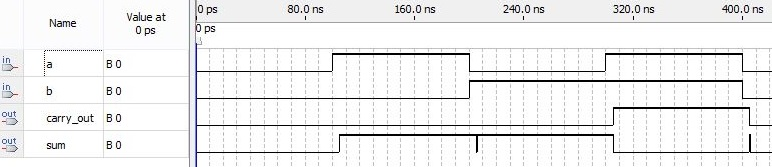
\includegraphics[scale=0.6]{pictures/Oevelse1/Half_adder/Dataflow_timing_simulation.jpg}
	\caption{Half-adder - Dataflow Timing Simulation}
	\label{fig:HaDatalfowTimingSim}
\end{figure}
\begin{figure}[h]
	\centering
	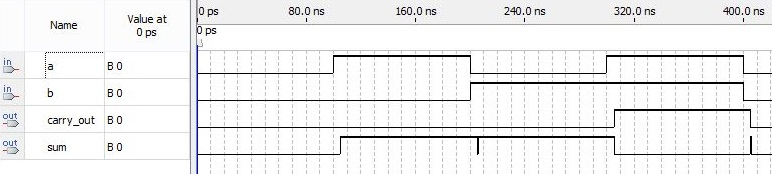
\includegraphics[scale=0.6]{pictures/Oevelse1/Half_adder/Structural_timing_simulation.jpg}
	\caption{Half-adder - Structural Timing Simulation}
	\label{fig:HaStructuralTimingSim}
\end{figure}
	\newpage
	Som det ses på figurerne, forekommer der nogle spikes på funktionerne. Dette skyldes static hazard, da de "gates" vi bruger i vores half-adder, vil have en lille tidsforskydning fra hinanden, og dermed kan give forkerte resultater i brøkdelen af et nanosekund, som det eksempelvis ses når både a-signalet og b-signalet ændrer status.
	\item[4)] 
	For at undgå disse spikes laver vi en functional simulation. Denne slags simulering tager højde for static hazard, og optimerer diagrammet til at vise et "perfekt" resultat.\\
	Figur \ref{fig:HaDataflowFunctionalSim}, \ref{fig:HaBehavioralFunctionalSim} og \ref{fig:HaStructuralFunctionalSim} viser denne type simulering.\\
\begin{figure}[h]
	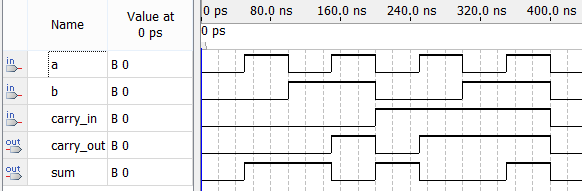
\includegraphics[scale=0.6]{pictures/Oevelse1/Half_adder/Dataflow_functional_simulation.jpg}
	\caption{Half-adder - Dataflow functional Simulation}
	\label{fig:HaDataflowFunctionalSim}
\end{figure}
\begin{figure}[h]
	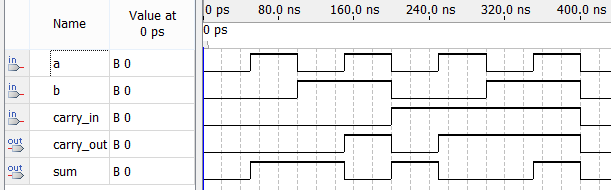
\includegraphics[scale=0.6]{pictures/Oevelse1/Half_adder/Behavioral_functional_simulation.jpg}
	\caption{Half-adder - Behavioral functional Simulation}
	\label{fig:HaBehavioralFunctionalSim}
\end{figure}
\begin{figure}[h]
	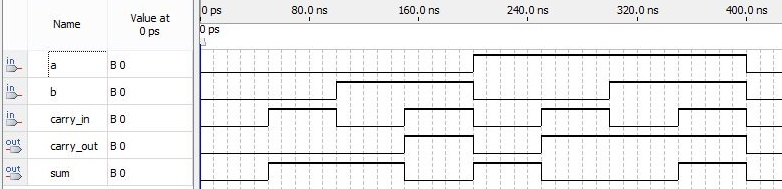
\includegraphics[scale=0.6]{pictures/Oevelse1/Half_adder/Structural_functional_simulation.jpg}
	\caption{Half-adder - Structural functional Simulation}
	\label{fig:HaStructuralFunctionalSim}
\end{figure}
	\newpage
\end{enumerate}